\section{Stage 1}

\begin{center}\rule{3in}{0.4pt}\end{center}

\$\$LMS = \textbackslash{}frac\{LMS\}\{lens + macula\}\$\$

\begin{figure}[htbp]
\centering
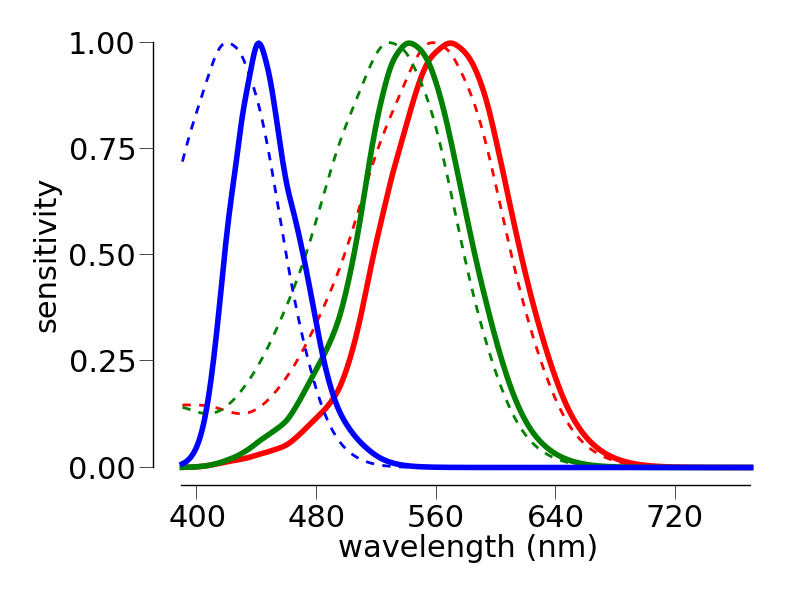
\includegraphics{../presentations/static/figures/colorModel/fundamentals.png}
\caption{somethings}
\end{figure}

\section{Stage 2}

\begin{center}\rule{3in}{0.4pt}\end{center}

\$\$L\_\{channel\} =
\textbackslash{}int\_\{\textbackslash{}lambda=390\}\^{}\{750\}
\textbackslash{}Big(w(q S\_\{\textbackslash{}lambda\} + (1-l)
M\_\{\textbackslash{}lambda\} + l L\_\{\textbackslash{}lambda\}) -
L\_\{\textbackslash{}lambda\}\textbackslash{}Big)
d\textbackslash{}lambda = 0\$\$

\$\$M\_\{channel\} =
\textbackslash{}int\_\{\textbackslash{}lambda=390\}\^{}\{750\}
\textbackslash{}Big(w(q S\_\{\textbackslash{}lambda\} + (1-l)
M\_\{\textbackslash{}lambda\} + l L\_\{\textbackslash{}lambda\}) -
M\_\{\textbackslash{}lambda\}\textbackslash{}Big)
d\textbackslash{}lambda = 0\$\$

\subsection{25\% L}

\begin{figure}[htbp]
\centering
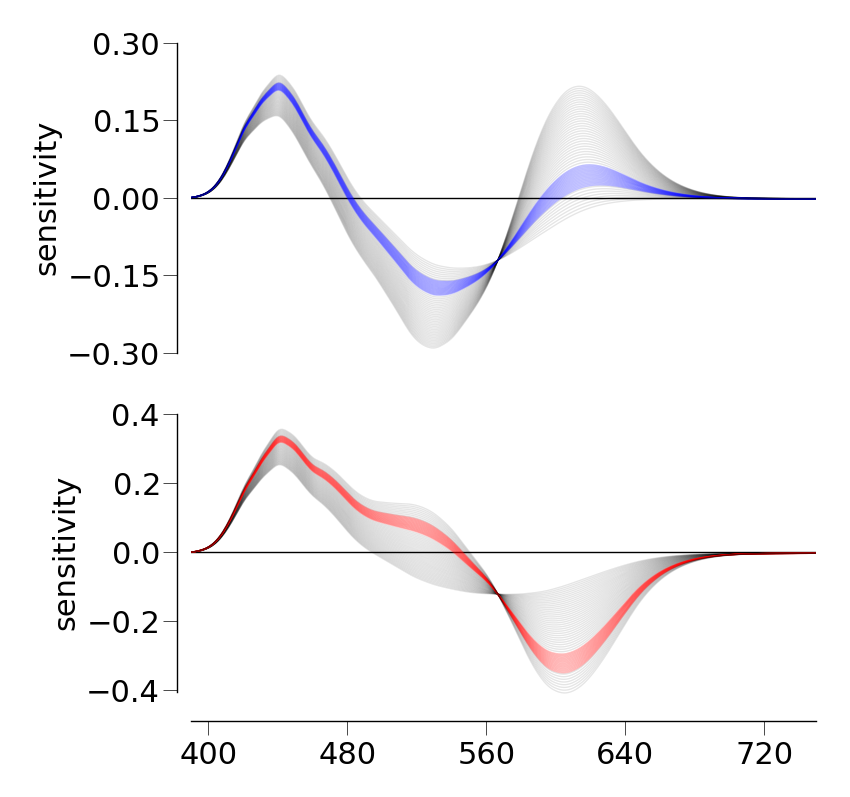
\includegraphics{../presentations/static/figures/colorModel/familyLMS_25L.png}
\caption{somethings}
\end{figure}

\subsection{75\% L}

\begin{figure}[htbp]
\centering
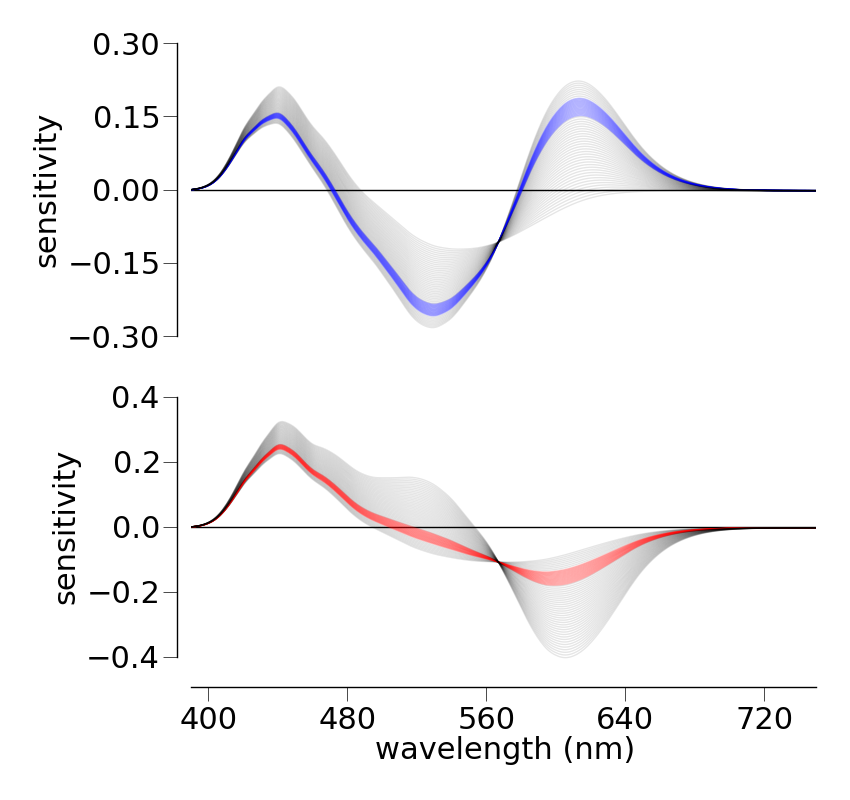
\includegraphics{../presentations/static/figures/colorModel/familyLMS_75L.png}
\caption{somethings}
\end{figure}

\section{Stage 3}

\begin{center}\rule{3in}{0.4pt}\end{center}

\$\$RG= \textbackslash{}sum\_\{m=0\}\^{}\{100\}
\textbackslash{}sum\_\{l=0\}\^{}\{100\} L\_\{channel\_\{l,m\}\} *
P(S\textbar{}l)\$\$

\$\$BY = \textbackslash{}sum\_\{m=0\}\^{}\{100\}
\textbackslash{}sum\_\{l=0\}\^{}\{100\} M\_\{channel\_\{l,m\}\} *
P(S\textbar{}l)\$\$

\$\$P(S\textbar{}l) = \textbackslash{}binom\{n\}\{L\} P\_\{l\}\^{}\{L\}
(1 - P\_\{l\})\^{}\{n - L\},\$\$

where \$n = L + M\$.

\begin{figure}[htbp]
\centering
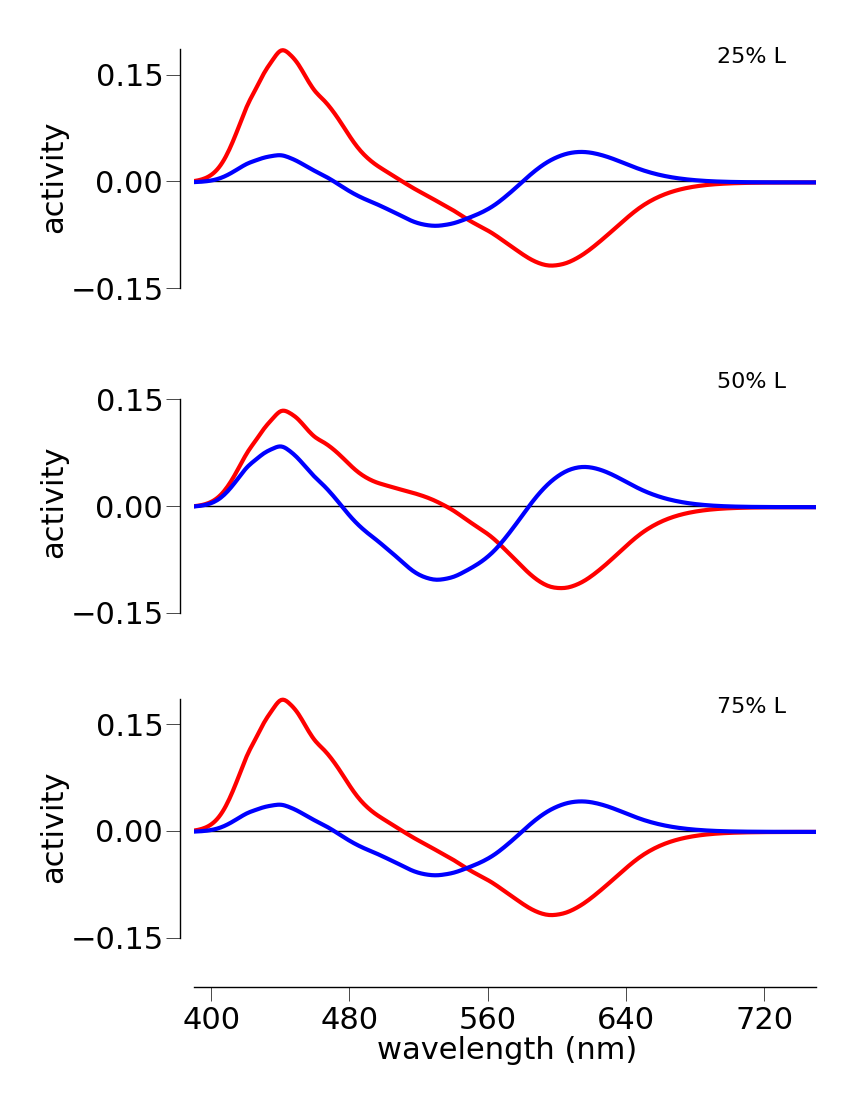
\includegraphics{../presentations/static/figures/colorModel/PercentL.png}
\caption{somethings}
\end{figure}

\begin{figure}[htbp]
\centering
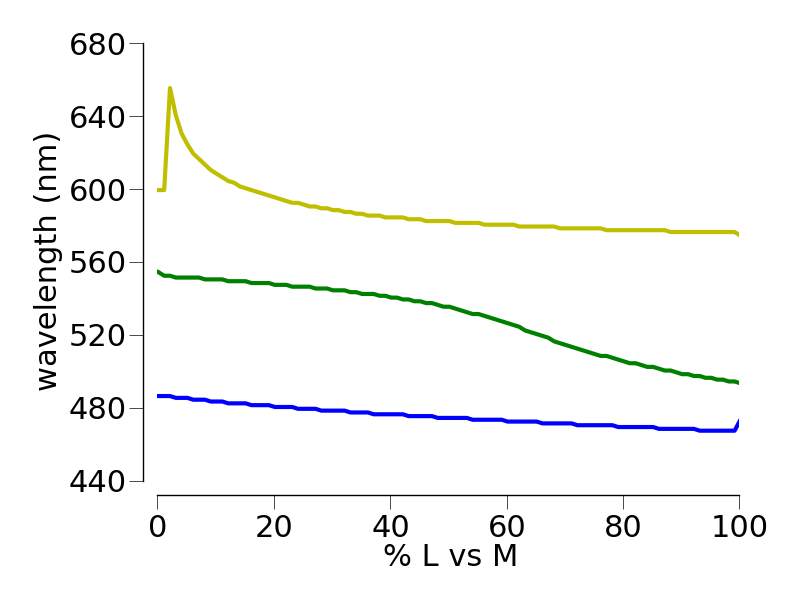
\includegraphics{../presentations/static/figures/colorModel/uniqueHues.png}
\caption{somethings}
\end{figure}

\section{Unique hues, LM ratio comparison}

\begin{center}\rule{3in}{0.4pt}\end{center}

\begin{figure}[htbp]
\centering
\includegraphics{../presentations/static/figures/colorModel/uniqueHues_LMcomparison.png}
\caption{somethings}
\end{figure}

\begin{figure}[htbp]
\centering
\includegraphics{../presentations/static/figures/colorModel/Volbrecht1997.gif}
\caption{somethings}
\end{figure}
